\documentclass{article}

\usepackage{amsfonts}
\usepackage[all]{xy}
\usepackage{amssymb}
\usepackage{amsmath}
\usepackage{mathrsfs}
\usepackage{amsthm}
\usepackage{enumerate}
\usepackage[hidelinks]{hyperref}
\usepackage{ulem}
\usepackage{tikz}  
\usetikzlibrary{arrows.meta}%画箭头用的包

\usepackage{geometry}
\geometry{a4paper,left=1cm,right=5cm,top=1cm,bottom=2cm}

\newtheorem{defn}{Definition}[section]
\newtheorem{prop}[defn]{Proposition}
\newtheorem{lem}[defn]{Lemma}
\newtheorem{thm}[defn]{Theorem}
\newtheorem{cor}[defn]{Corollary}
\newtheorem{rmk}[defn]{Remark}
\newtheorem{fact}[defn]{Fact}
\newtheorem{problem}{Problem}
\newtheorem*{ques}{Question}

\setcounter{section}{0}

\title{Log Sarkisov Program}
\date{}
\begin{document}
	\maketitle
	\tableofcontents
	\newpage
\section{Introduction}
\subsection{Main theorem}
Let $ (V,B_V) $ be an $ \mathbb{Q} $-factorial klt pair. Recall by BCHM, 
\begin{itemize}
	\item If  $ K_V+B_V $ is $ \mathbb{R} $-cartier and not pseudo-effective, then we can run MMP with scaling and  end with a Mori fibre space (MFS). 
	\item If $ K_V+B_V $ is $ \mathbb{R} $-cartier pseudo-effective and either $ B_V $ or $ K_V+B_V $ is big, then we can run MMP with scaling and end with a mininal model.
	\item These hold for relative case.
\end{itemize}
\begin{cor}\label{extraction}
	(Birational base case): Let $ (X,B) $ be a klt pair and $ S $ be any set of exceptional divisors such that  contains only exceptional divisors $ E $ of dicrepancy $ a(E;X,B)\leqslant 0 $. Then there is a birational morphism $ f:Z\to X $ and a $ \mathbb{Q} $-divisor $ B_Z $ such that:
	\begin{enumerate}
		\item $ (Z,B_Z) $ is klt;
		\item $ E $ is an exceptional divisor for $ f $ iff $ E\in S $;
		\item $ B_Z=\sum-a(E;X,B) $ and $ f_*B_Z=B $ and $ K_Z+B_Z=f^*(K_X+B) $.
	\end{enumerate} 
\end{cor}
In particular, if we take $ S $ containing all such divisors, then $ (Z,B_Z) $ is called \textbf{terminalization} of $ X $; if take $ S $ containing only one such divisor, then $ f:(Z,B_Z)\to X $ is called a \textbf{divisorial extraction}.	
\begin{proof}
	Consider log resolution $ \pi:V\to X $ and 
	$$ K_V+\pi^{-1}_*B+\sum a_iE_i +\sum a_jE_j=\pi^*(K_X+B)+\sum f_kE_k$$
	with $ a_i,a_j\geqslant 0, f_k<0 $ and $ S=\{ E_i \} $
	Then let $ B_V=\pi^{-1}_*B+\sum a_iE_i +\sum (a_j+\epsilon)E_j+\sum \epsilon F_k $ such that $ (V,B_V) $ is klt, then 
	$$ K_V+B_V=\pi^*(K_X+B)+\sum \epsilon E_j+\sum (\epsilon+f_k)E_K $$
	Run relative $ (K_V+B_V) $-MMP on $ V $ over $ X $ and end with relative minimal model $ (Z,B_Z)\to X $.
\end{proof}
However, the outputs of a MMP may be different:
\begin{defn}
	Two or more pairs $ \{(X_i,B_i)\} $ is MMP-related if they are outputs of $ (K+B) $-MMP over $ \mathrm{Spec}\,\mathbb{C} $ from a nonsingular  projective variety $ V $ and  boundary $ B_V $ with only normal crossing.
\end{defn}
\begin{rmk}
	Suppose $(X,B) $ and $ (X',B') $ are two  outputs of MMP on a klt pair $ (W,B_W) $, then take a log resolution $ \pi:W':\to W $ such that $ \sigma:W'\to X $ and $ \sigma':W'\to X' $ are morphisms. Furthermore, suppose
	$$ K_{W'}+\pi_*^{-1}B_W+E=\pi^*(K_W+B_W)+F $$
	where $ E,F $ are effective $ \pi $-excpetional divisors with no common component, and coefficients of $ E $ are less than $ 1 $. Let $ B_{W'}=\pi_*^{-1}B_W+E $, then $ f:(X,B)\to S $ and $ f':(X',B')\to S' $ are also  outputs of MMP on $ (W',B_{W'}) $. By Further blowing up, we may assume components of $ B_{W'} $ are disjoint, and hence $ (W',B_{W'}) $ is terminal (This does not hold for dlt pairs).  We can replace $ (W,B_W) $ by log smooth pair $ (W',B_{W'}) $. 
\end{rmk}

For mininal model case, we have
\begin{thm}
	(Yujiro Kawamata, 2008)
	
	Let $ (V,B_V) $ be an $ \mathbb{Q} $-factorial terminal  pair. Suppose $ (X,B) $ and $ (X',B') $ are two minimal models of $ (V,B_V) $, then the birational map 
	$$ X\dashrightarrow X' $$
	may factored as a sequence of $ (K+B) $-flops.
\end{thm}
For MFS, comes  the main theorem:
\begin{thm}
	Let $ f:(X,B)\to S,f':(X',B')\to S' $ be two $ \mathbb{Q} $-factorial log MFS  with only klt singularities and MMP-related, inducing a birational map:
	$$ \xymatrix{
		(X,B)\ar[d]_f\ar@{.>}[r]^\Phi&(X',B')\ar[d]^{f'}\\
		S&S'} $$
	Then $ \Phi  $ is composition  of links of  four types:
	
	$ \textbf{I} : \xymatrix{
		&Z\ar[ld]_p\ar@{.>}[r]^{flips}&X_1\ar[dd]^{f_1}\\
		X\ar[d]_f&&\\
		S &&S_1\ar[ll]}$
	$ \textbf{II} : \xymatrix{
		&Z\ar[ld]_p\ar@{.>}[r]^{flips}&Z'\ar[dr]^{q}&\\
		X\ar[d]&&&X_1\ar[d]_{f_1}\\
		S\ar@{=}[rrr]&&&S_1} $
	
	$ \textbf{III} :\xymatrix{
		X\ar[d]_f\ar@{.>}[r]^{flips}&Z\ar[rd]^{p}&\\
		S\ar[dr]&&X_1\ar[d]^{f_1}\\
		&T&S_1\ar[l]_\sim}$
	$  \textbf{IV}:\xymatrix{
		X\ar[d]_f\ar@{.>}[rr]^{flips}&&X_1\ar[d]^{f_1}\\
		S\ar[dr]&&S_1\ar[dl]\\
		&T &}$

	Here, all $ f:(X,B)\to S $ and $ f_1:(X_1,B_1)\to S_1 $ are log MFS, and all $ p,q $ are divisorial contractions, and all dash arrows are composition of flips (flops). 
\end{thm}
\begin{rmk}
	These links appear naturally when playing relative 2-ray games.
\end{rmk}
	\begin{itemize}
		\item For terminal threefolds:
		
		Factoring birational maps of threefolds after Sarkisov, Alwssio Corti, 1995;
		\item For dlt surface (and $ \mathrm{Aut}(\mathbb{A}^2) $):
		
		 Sarkisov program for log surfaces, Takahashi, 1995;
		\item For klt threefolds:
		
		Log Sarkisov program, Andrea Bruno and Kenji Matsuki, 1996
		\item For (g)klt pairs:
		
		The minimal model program for log general type, Christopher D. Hacon, 2013 (note);
		
		Sarkisov program for generalized pairs, Jihao Liu, 2021
		\item Another proof:
		
		The Sarkisov program, Christopher D. Hacon and James Mckernan, 2013;
		
		The Sarkisov program on log surfaces, Keisuke Miyamoto, 2019 (arkiv)
	\end{itemize}
\subsection{Example} 
 $ \mathrm{Aut} (\mathbb{A}^2) $

Let $ \phi: \mathbb{P}^2\dashrightarrow\mathbb{P}^2 $ be a birational map induced by an automorphism of $ \mathbb{A}^2 $. Then consider the dlt pairs $ (X,B)=(\mathbb{P}^2,H) $, $ (X',B')=(\mathbb{P}^2,H) $. Takahashi shows that there are only links of type II in such Sarkisov program, and can be described as toric varieties. Each link induces a map between $ \mathbb{A}^2 $ of one of the forms
\begin{enumerate}
	\item Identity;
	\item $ (x,y)\to (x,y+ax) $;
	\item $ (x,y)\to (x,y+ax^k), k>1 $;
	\item $ (x,y)\to (y,x) $.
\end{enumerate}
\subsection{Ideas of the proofs}
We are going to replace $ X_i $ by $ X_{i+1} $ inductively, where $ X_i\dashrightarrow X_{i+1} $ is composition of divisorial extraction, extremal contraction and flips, such that $ X_{i+1} $ is closer to $ X' $ than $ X_i $. Therefore, we need to mark the position of the pairs:

Suppose $ \Phi $ is defined on $ U\subset X $, then $ \mathrm{codim}\,(X-U,X)\geqslant 2 $ since $ X $ is normal. If we fix a very ample divisor $ A'  $ on $ S' $ and a sufficiently large and divisible integer $ \mu'>1 $ such that 
$$ \mathcal{H}'=|-\mu' (K_{X'}+B') +f'^*A'| $$
is a very ample complete linear system on $ X' $ (over $ \mathrm{Spec}\,\mathbb{C} $),  inducing an embedding into $ \mathbb{P}^N $ for some $ N $.  Let $ (V,B_V) $ be a common log resolution of $ X $ and $ X' $  with projective birational morphism $ p:V\to X$,   $q:V\to X' $ and $p_*B_V=B, q_*B_V=B' $,
$$ \xymatrix{
&V\ar[ld]_p\ar[rd]^{q}&&\\
X\ar[d]\ar@{.>}[rr]&&X'\ar[d]\ar[r]^{\mathcal{H}'}&\mathbb{P}^N\\
S&&S'} $$ 
take a general divisor $ H'\in \mathcal{H}' $ such that 
$$ H_V:=q^*H'=q^{-1}_*H' $$ Then the pair $ (X',B'+\frac{1}{\mu'}H') $ is a minimal model for $ (V,B_V+\frac{1}{\mu'}H_V) $, and $ S' $ is an ample model. This shows the position of  $ (X',B') $ w.r.t. $ V $.
\begin{enumerate}
	\item Orginal method: Fix a general divisor $ H' $ . For each $ X_i $, find a common resolution $ V_i $ for $ X_i $ and $ X' $. Mark the position of $ (X',B') $ by $ H' $ w.r.t. $ V_i $ . Let $ H_i $ be homaloidal transform $ p_*q^*H' $ of $ H' $. In fact, $ H_i=\phi^{-1}_*H' $. Note that $ (X_i,B_i+\frac{1}{\mu'}H_i) $ generally is not a minimal model.
	
	Then we fine $ (X_{i+1},B_{i+1},H_{i+1}) $ by run certain MMP (2-ray games) on $ X_i $.
	\item Double sacling: Assume they are outputs of a log smooth terminal pair $ (W,B_W) $. Mark the positions for both pairs w.r.t. $ (W,B_W) $: Find a ample divisor $ A $($ A' $) on $ S $($ S' $) such that $ C=-(K_X+B)+f^*A $ ($ H'=-(K_{X'}+B')+f^{'*}A' $) is ample, and find $ C_W $($ H_W $) on $ W $ such that $ p^*C=p^{-1}_*C=C_W $ ($ q^*H'=q^{-1}_*H'=H_W $). 
	$$ \xymatrix{
		&(W,B_W+c_iC_W+h_iH_W)\ar[d]\ar[ld]_p\ar[rd]^{q}&\\
		X\ar[d]\ar@{.>}[r]&X_i\ar@{.>}[r]\ar[d]&X'\ar[d]\\
		S&S_i&S'} $$ 
	Then $ (X,B+C) $/$ (X',B'+H') $ is a minimal model for $ (W,B_W+C_W) $/$ (W,B_W+H_W) $. For each link, $ (X_i,B_i+c_iC_i+h_i+H_i) $ is a minimal model for $ (W,B_W+c_iC_W+h_iH_W) $ with $ 1\geqslant c_i\geqslant c_{i+1}\geqslant 0 $ and $ 0\leqslant h_i\leqslant h_{i+1}\leqslant 1 $. 
\end{enumerate}


\section{Original method}
 
\subsection{Sarkisov degree}
Difference between terminal case $ X\to S $ and klt case $ (X,B)\to S $: for every $ X_i,Z_i,Z_i' $ and $ V_i $, we have to find a corresponding boundary:

\begin{lem}
	Let $ \{(X_l,B_l)\} $ be a finite family of $ \mathbb{Q} $-factorial klt pairs, then TFAE:
	\begin{enumerate}[(a)]
		\item They are MMP-related;
		\item There is a nonsingular pair $ (V,B_V) $ with snc boundary, and projective birational morphisms $ f_l:V\to  X_l $ dominating each $ X_l $, such that $ f_{l*}B_V=B_l $ and
		$$ K_V+B_V=f_l^*(K_{X_l}+B_l)+\sum_{exceptional}{a_{li}E_{li}} $$
		with $ a_{li}>0 $ for all $ f_i $-exceptional divisors;
		\item For any two pairs $ (X,B=\sum_ib_iB_i),(X',B'=\sum _jb_j'B_j') $ in the family,  $ a(B_i;X',B')\geqslant -b_i $ and strict inequality holds iff $ B_i $ exceptional over $ X' $, and $ a(B'_j;X,B)\geqslant -b'_j $ and strict inequality holds iff $ B'_j $ exceptional over $ X $
	\end{enumerate}
\end{lem}
Let $ K=K(X) $ be the function field, and let $ \{\nu\} $ be the set of discrete valutions. 
\begin{defn}
	Fix a function 
	$$ \theta:\{\nu\}\to [0,1)_\mathbb{Q} $$
	Then we can construct a collection $ \mathcal{C}_\theta $ of pairs  associated to $ \theta $, consists of klt pairs $ (X,B=\sum a_iB_i) $ satisfying
	\begin{enumerate}
		\item $ a_i=\theta(B_i) $;
		\item $ a(E;X,B)>-\theta(E) $ for all $ E $ exceptional over $ X $.
	\end{enumerate} 
\end{defn}
A pair $ (X,B) $ is $ \theta $-terminal ($ \theta $-canonical) if $ a(E;X,B)>(\geqslant)-\theta(E) $ for all $ E $ over $ X $.


In particular, for our problem we can take a category as follows:
\begin{prop}\label{cat}
	Let $ f:(X,B)\to S,f':(X',B')\to S' $ be two $ \mathbb{Q} $-factorial log MFS  with only klt singularities and MMP-related, inducing a birational map:
	$$ \xymatrix{
		(X,B)\ar[d]_f\ar@{.>}[r]^\phi&(X',B')\ar[d]^{f'}\\
		S&S'} $$
	Suppose  $ B=\sum_ib_iB_i+\sum_jd_jD_j $ and $ B'=\sum_jd_j'D_j+\sum_kb_k'B_k' $, where $ B_i $ are divisors on $ X $ but not on $ X' $, $ B_k' $ are divisors on $ X' $ but not on $ X $, and $ D_j $ are divisors on both $ X $ and $ X' $. By lamma above, $ d_j=d_j' $. Take a rational number $ \epsilon=1-\delta $ such that $ 0<b_i,d_j,b_k', -\mathrm{discrep}(X,B),-\mathrm{discrep}(X',B')<\epsilon<1 $, and fix the function $ \theta:\{\nu\}\to [0,1)_\mathbb{Q} $ as following:
	\begin{itemize}
		\item $ \theta(B_i)=b_i, \theta(D_j)=d_j,\theta(B_k')=b_k'$;
		\item $ \theta(E)=\epsilon $ if $ E $ is exceptional on both $ X $ and $ X' $;
		\item $ \theta(D)=0 $ if $ D $ is a divisor on both $ X $ and $ X' $, but not a componet of $ B $ or $ B' $.
	\end{itemize}
	Then the collection $ \mathcal{C}_\theta $ satisfies
	\begin{enumerate}[1)]
		\item $ (X,B) $ and $ (X',B') $ belongs to $ \mathcal{C}_\theta $;
		\item For any finitely many klt pairs $ \{(X_l,B_l)\} $ in $ \mathcal{C}_\theta $, there is an object $ (Z,B_Z)\in \mathcal{C}_\theta $ and projective birational morphisms $ Y\to X_l $ dominating each	$ X_l $ as a process of $ (K+B) $-MMP over $ X_l $ (thus over $ \mathrm{Spec}\,\mathbb{C} $);
		\item Any $ (K+B) $-MMP starting from an object in $ \mathcal{C}_\theta $ stays inside $ \mathcal{C}_\theta $, and so does any $ (K+B+cH) $-MMP where $ H $ is base point free and $ c\in \mathbb{Q}_{>0} $. 
	\end{enumerate}
\end{prop}

\begin{rmk}
	\begin{itemize}
		\item All the objects in the collection $ \mathcal{C}_\theta $ are $ \delta $-lc;
		\item In particular, if we take $ \theta\equiv 0 $, then this is the terminal case.
	\end{itemize}	
\end{rmk}


Suppose $ \Phi $ is defined on $ U\subset X $, then $ \mathrm{codim}\,(X-U,X)\geqslant 2 $ since $ X $ is normal. If we fix a very ample divisor $ A'  $ on $ S' $ and a sufficiently large and divisible integer $ \mu'>1 $ such that 
$$ \mathcal{H}'=|-\mu' (K_{X'}+B') +f'^*A'| $$
is a very ample complete linear system on $ X' $ over $ \mathrm{Spec}\,\mathbb{C} $,  inducing an embedding into $ \mathbb{P}^N $ for some $ N $. Pull back $ (\Phi|_U)^*\mathcal{H}' $ of the linear system is a base point free linear system on $ U $, and can be extended  to a movable linear system on $ X $, which coincides with strict transform $ \mathcal{H}:=\Phi^{-1}_*\mathcal{H}' $ , and induces a rational map $ X\dashrightarrow \mathbb{P}^N $. Let $ (V,B_V) $ be a common log resolution of $ X $ and $ X' $ in $ \mathcal{C}_\theta $ with projective birational morphism $ \sigma:V\to X$,   $\sigma':V\to X' $ and $\sigma_*B_V=B, \sigma'_*B_V=B' $, denote
$$ \mathcal{H}_V:=\sigma'^*\mathcal{H}' $$
and then 
$$ \mathcal{H}:=\Phi^{-1}_*\mathcal{H}'=\sigma_*\mathcal{H}_V $$
Furthermore, if $ \mathcal{H} $ is not base point free, then
$$ \sigma^*\mathcal{H}=\mathcal{H}_V+F $$
where $ \sum f_lF_l=F\geqslant0 $ is the fixed part, and $ \sigma(\mathrm{Supp}\,F)\subset X-U $. 

Take a general member $ H' $ of the linear system $ \mathcal{H}' $ such that $ H_V:=\sigma'^*H'=\sigma'^{-1}_*H'\in \mathcal{H}_V $, and let $ H:=\Phi^{-1}_*H'=\sigma_*H $, then $ \sigma^*H=H_V+F $. Since $ \rho(X/S)=1 $ (($\rho( X'/S')=1 $), any effective divisor on $ X $ ($ X' $) is $ f $($ f' $)-ample, including $ H $($ H' $). 

Fixing a collection $ \mathcal{C}_\theta $ as in \ref{cat}. 
\begin{defn}
	Sarkisov degree of $ (X,B) $ w.r.t. $ H $ ($ \mathcal{H} $) in $ \mathcal{C}_\theta $ is a triple $ (\mu,\lambda,e) $ orderd lexicographically:
	\begin{itemize}
		\item Nef threshold $ \mu $: Let $ C\subset X  $ be a curve contracted by $ f $, then 
		$$ \mu:=-\frac{H.C}{(K_X+B).C} $$
		i.e. $ K_X+B+\frac{1}{\mu} H \equiv_S0$ and hence $ f^*A=K_X+B+\frac{1}{\mu} H $ for some $ \mathbb{Q} $-divisor on $ S $;
		\item $ \theta $-canoncial threshold $ \lambda $: Take a common log resolution  $ (V,B_V)\in \mathcal{C}_\theta $ with $ B_V=\sum \theta(E)E $ and projective birational morphisms $ \sigma:V\to X $, $ \sigma':V\to X' $. Take a general member $ H'\in \mathcal{H}' $ such that $ H_V:=\sigma'^{-1}_*H'=g^{-1}_*H $. Suppose $ \sigma^*H=H_V+\sum f_lF_l $ with $ \sum f_lF_l $ effective and $ \sigma $-exceptional (by negativity lemma), then we have ramification formulars
		$$ K_V+B_V=\sigma^*(K_X+B+cH)+\sum a_lE_l  $$
		$$ K_V+B_V+cH_V=\sigma^*(K_X+B+cH)+\sum(a_l-cf_l)E_l $$
		where $ \sum a_lE_l $ is effective and supported on $ \mathrm{Exc}\,\sigma $.   Let
		$$ \lambda:=\max\{ \frac{f_l}{a_l}\} $$
		This is independent on the choice of log resolution. In fact $ \frac{1}{\lambda} $ is called $ \theta $-canonical threshold w.r.t. $ (X,B;H) $, i.e.
		$$ \frac{1}{\lambda}:=\max\{c:a(E;X,B+cH)\geqslant-\theta(E) ,E\text{ exceptionl over }X \}$$ 
		If $ \mathcal{H} $ is base point free, then $ \sum f_lF_l=0 $ and $\sum(a_l-cf_l)E_l\geqslant 0  $ always holds, in which case $ \lambda=0 $ by definition;
		\item $ e=0 $ if $ \mathcal{H} $ is base point free (and hence $ \lambda=0 $), otherwise 
		$$ e=\#\{E_i; E_i \text{ is }\sigma\text{-exceptional and } a(E;X,B+\frac{1}{\lambda} H)=-\theta(E) \} $$
		or equivalently in the formular 
		$$ K_V+B_V+\frac{1}{\lambda} H_V=\sigma^*(K_X+B+\frac{1}{\lambda} H)+\sum(a_l-cf_l)E_l $$
		$ e $ is the number of components in $ E-\frac{1}{\lambda} F $ with coefficient $ 0 $. 
	\end{itemize}
\end{defn}


\subsection{Flow chart}
\textbf{Start:}
\begin{enumerate}[(A)]
	\item If $ \lambda\leqslant\mu $:
	
	If $ K_X+B+\frac{1}{\mu}H $ is nef, then we stop;
	
	If $ K_X+B+\frac{1}{\mu}H $ is not nef: The idea is running $ (K_X+B+\frac{1}{\mu}H) $-MMP on $ X $, but keep it simple, i.e. play 2-ray game:
	
	Suppose $ f $ is the contraction w.r.t. a $ (K_X+B) $-negative extremal ray $ R= \overline{NE}(X/S) $, then $ (K_X+B+\frac{1}{\mu}H).R=0 $ by definition of $ \mu $.  Take an extremal ray $ P\in \overline{NE}(X) $ such that $ (K_X+B+\frac{1}{\mu}H).P<0 $ and $ F:=P+R $ is an extremal face. Take  a contraction $ g:X\to T $ w.r.t. to $ F $ factorizing through $ f:X\to S $: 
	$$ \xymatrix{
		X\ar[d]_f\ar[ddr]^g&\\
		S\ar[dr]&\\
		&T }$$
	$ (X,B+\frac{1}{\mu}H) $ is klt, and $ \rho(X/T)=2 $, thus we can  run $ (K_X+B+\frac{1}{\mu}H) $-MMP on $ X $ over $ T $ as a 2-ray game:  Start with a finite sequence of flips, and the first non-flip contraction is either a divisorial contraction or a fibering contraction, or it ends as a relative minimal model. 
	\begin{enumerate}[1)]
		\item If after finitely many flips $ X\dashrightarrow Z $, first non-flip contraction is a divisorial contraction $ p:Z\to X_1\xrightarrow{g_1}T $, and the MMP ended with a MFS.  Since $ \rho(X_1/T)=1 $, there is no further flips or divisorial contraction, thus must be followed by a fibering contraction $ f_1:X_1\to Y $ with $ Y\xrightarrow{\sim}T $.
		$$ \xymatrix{
			X\ar[d]_f\ar[ddr]^g\ar@{.>}[r]^{flips}&Z\ar[rd]^{p}&\\
			S\ar[dr]&&X_1\ar[d]^{f_1}\ar[ld]_{g_1}\\
			&T&Y\ar[l]_\sim}$$
		Furthermore, denote $ H_1 $ the strict transform of $ H $ and $ H' $. Since $ \rho(X_1/Y)=1 $ and $ H_1 $ is effective, $ H_1 $ is $ f_1 $-ample, thus $ (K_{X_1}+B_1) $ is $ f_1 $-negative and $ (X_1,B_1)/Y $ is a log MFS.  Take $ S_1=Y $.
		$$ \xymatrix{
			X\ar[d]_f\ar@{.>}[r]^{flips}&Z\ar[rd]^{p}&\\
			S\ar[dr]&&X_1\ar[d]^{f_1}\\
			&T&S_1\ar[l]_\sim}$$
		This is a link of type III. 	
		\item If after finitely many flips $ X\dashrightarrow X_1 $, first non-flip contraction is a fibering contraction $ f_1:X_1\to Y  $
		$$ \xymatrix{
			X\ar[d]_f\ar[ddr]^g\ar@{.>}[rr]^{\psi_1}&&X_1\ar[d]^{f_1}\ar[ddl]_{g_1}\\
			S\ar[dr]&&Y\ar[dl]\\
			&T &}$$
		Same as above, $ (X_1,B_1)/Y $ is a log MFS. Take $ S_1=Y $
		$$ \xymatrix{
			X\ar[d]_f\ar@{.>}[rr]^{\psi_1}&&X_1\ar[d]^{f_1}\\
			S\ar[dr]&&S_1\ar[dl]\\
			&T &}$$
		this is a link of type IV. 
		\item If after finitely many flips $ X\dashrightarrow Z $, first non-flip contraction is a divisorial contraction $ p:Z\to X_1\xrightarrow{g_1}T $ with 
		$$ K_Z+B_Z+\frac{1}{\mu}H_Z=p^*(K_{X_1}+B_1+\frac{1}{\mu}H_1)+eE $$
		where $ e>0 $ and the MMP ended with a relatively log minimal model. Since  $ \rho(X_1/T)=1 $, $ (X_1,B_1+\frac{1}{\mu}H_1) $ must be the log minimal model.
		$$ \xymatrix{
			X\ar[d]_f\ar[ddr]^g\ar@{.>}[r]^{flips}&Z\ar[rd]^{p}&\\
			S\ar[dr]&&X_1\ar[dl]_{g_1}\\
			&T&}$$
		Claim that the only ray of $ \overline{NE}(X_1/T) $ is $ (K_{X_1}+B_1+\frac{1}{\mu}H_1) $-trival. Indeed, take a curve $ C_1\subset X_1 $ contracted by $ g_1 $ away from indeterminacy of $ X_1\dashrightarrow X $ ( union of image of exceptional divisor of $ p $ and all flipped curves) and not contained in the base locus of $ \mathcal{H}_1 $, then $ C $ can be considered also to lie on $ X $ and contracted by $ g $ and $ H_1.C\geqslant 0 $.  The union of  indeterminacy locus and base locus of $ \mathcal{H}_1 $ is a closed subset of $ X_1 $, thus suppose there is an open subset $ U_1 $ of $ X_1 $ avioding that closed subset, and  isomorphic to an open subset $ U $ of $ X $. Thus $ [C]\in F $ and
		\begin{equation*}
			\begin{aligned}
				0\geqslant& (K_X+B+\frac{1}{\mu}H).C_X\\
				=&(K_Z+B_Z+\frac{1}{\mu}H_Z).C_Z\\
				\geqslant&(K_Z+B_Z+\frac{1}{\mu}H_Z-eE).C\\
				=&(K_{X_1}+B_1+\frac{1}{\mu}H_1).C\geqslant 0\\
			\end{aligned}
		\end{equation*}
		Therefore $ (K_{X_1}+B_1+\frac{1}{\mu}H_1).C_1=0 $. Furthermore, $ H_1 $ is effective, thus is $ g_1 $-ample, and hence $ (K_{X_1}+B_1) $ is $ g_1 $-negative, and $ (X_1,B_1)/T $ is a log MFS. Take $ S_1=T $
		$$ \xymatrix{
			X\ar[d]_f\ar@{.>}[r]&Z\ar[rd]^{p}&\\
			S\ar[dr]&&X_1\ar[d]^{f_1}\\
			&T&S_1\ar@{=}[l]}$$
		This is a link of type III. Since $ (K_{X_1}+B_1+\frac{1}{\mu}H_1) $ is trival on the ray $ R=\overline{NE}(X_1/S_1) $, we  have 
		$$ \mu=\mu_1 $$
		Notice that $ (X_1,B_1+\frac{1}{\mu}H_1) $ stays $ \theta $-canonical, we have
		$$ \lambda_1\leqslant \mu=\mu_1 $$
		Furthermore, $ \rho(X_1)=\rho(X)-1 $.
		\item If after finitely many flips $ X\dashrightarrow X_1 $, MMP ends with log minimal model $ (X_1,B_1+\frac{1}{\mu}H_1)/T $
		$$ \xymatrix{
			X\ar[d]_f\ar[ddr]^g\ar@{.>}[rr]^{flips}&&X_1\ar[ddl]_{g_1}\\
			S\ar[dr]&&\\
			&T &}$$
		Claim that there is a ray of $ \overline{NE}(X_1/T) $ is $ (K_{X_1}+B_1+\frac{1}{\mu}H_1) $-trival and $ (K_{X_1}+B_1) $-negative. Indeed, take a curve $ C\subset X_1 $ contracted by $ g_1 $ away from indeterminacy of $ X_1\dashrightarrow X $ ( union of all flipped curves) and not contained in the base locus of $ \mathcal{H}_1 $, then $ C $ can be considered also to lie on $ X $ and contracted by $ g $ and $ H_1.C\geqslant 0 $, thus $ [C]\in F $ and
		\begin{equation*}
			\begin{aligned}
				0\geqslant& (K_X+B+\frac{1}{\mu}H).C\\
				=&(K_{X_1}+B_1+\frac{1}{\mu}H_1).C\geqslant 0\\
				0> &(K_X+B+(\frac{1}{\mu}-t)H).C\\
				=&(K_{X_1}+B_1+(\frac{1}{\mu}-t)H_1).C\geqslant (K_{X_1}+B_1).C
			\end{aligned}
		\end{equation*}
		Take a contraction $ f_1:X_1\to S_1 $ w.r.t. $ (K_{X_1}+B_1) $-negative ray $ R=\mathbb{R}_{\geqslant 0}[C] $
		$$ \xymatrix{
			X\ar[d]_f\ar@{.>}[rr]&&X_1\ar[d]^{f_1}\\
			S\ar[dr]&&S_1\ar[dl]\\
			&T &}$$
		This is a link of type IV. Since $ (K_{X_1}+B_1+\frac{1}{\mu}H_1) $ is trival on the ray $ R=\overline{NE}(X_1/S_1) $, we  have 
		$$ \mu=\mu_1 $$
		Notice that $ (X_1,B_1+\frac{1}{\mu}H_1) $ stays $ \theta $-canonical, we have
		$$ \lambda_1\leqslant \mu=\mu_1 $$
	\end{enumerate}
	\item If $ \lambda>\mu $, then $ (X,B+\frac{1}{\mu}H) $ is not $ \theta $-canonical. Take a divisorial extraction $ p:(Z,B_Z,H_Z)\to (X,B,H) $ in $ \mathcal{C}_\theta $ w.r.t. $ K_X+B+\frac{1}{\lambda}H $, i.e. $ (Z,B_Z) $ is $ \theta $-terminal and $ p^*(K_X+B+\frac{1}{\lambda}H)=K_Z+B_Z+\frac{1}{\lambda}H_Z $ where $ B_Z=\sum\theta(E_\nu)E_\nu $ and $ E=\mathrm{Exc}\,p $ is a prime divisor on $ Z $.  Let $ H_Z=p^{-1}_*H $ be the strict transform of a general member $ H' $ of $ \mathcal{H}' $: 
	$$ \xymatrix{
		&Z\ar[ld]_p\ar[ldd]\\
		X\ar[d]&\\
		S} $$
	Run $ (K_Z+B_Z+\frac{1}{\lambda}H_Z) $-MMP on $ Z $ over $ S $, then it always ends with a MFS. Otherwise, there are two cases:
	\begin{enumerate}[a)]
		\item After finitely many flips $ Z\dashrightarrow Z' $, first non flip contraction is a divisorial contraction $ q:Z'\to X_1 $. Since $ \rho(X_1/S)=1 $, $ (X_1,B_1+\frac{1}{\lambda}H_1) $ must be the ending log minimal model.
		$$ \xymatrix{
			&Z\ar[ld]_p\ar[rdd]^{g}\ar@{.>}[rr]^{flips}&&Z'\ar[dr]^{q}&\\
			X\ar[drr]\ar@{.>}[rrrr]^{\psi_1}&&&&X_1\ar[dll]^{g_1}\\
			&&S&&} $$
		Let $ E_q=\mathrm{Exc}\,q $ be the exceptional divisor, then 
		$$ K_{Z'}+B_{Z'}+\frac{1}{\lambda}H_{Z'}=q^*(K_{X_1}+B_1+\frac{1}{\lambda}H_1)+aE_q \,(a>0)$$
		Take a curve $ C_X\subset X $ contracted by $ f $ and away from $ p(E) $ (thus can be considered to be a curve $ C_Z $ on $ Z $) and flipped curves (thus can be considered to be a curve $ C_{Z'} $ on $ Z' $) and $ E_q $ (thus $ E_q.C_Z\geqslant 0 $ ), then
		\begin{equation*}
			\begin{aligned}
				0\leqslant& (K_{X_1}+B_1+\frac{1}{\lambda}H_1).q_*C_{Z'} \text{ (it is a minimal model)}\\
				=&(K_{Z'}+B_{Z'}+\frac{1}{\lambda}H_1-aE_q).C_{Z'}\\
				=&(K_{Z}+B_{Z}+\frac{1}{\lambda}H_1-aE_q).C_{Z}\\
				\leqslant &(K_{Z}+B_{Z}+\frac{1}{\lambda}H_1).C_{Z}\\
				=&(K_X+B+\frac{1}{\lambda}H).C_X\\
				<&(K_{X}+B+\frac{1}{\mu}H).C_X  \,(\frac{1}{\lambda}<\frac{1}{\mu})\\
				=&0
			\end{aligned}
		\end{equation*} 
		Contraction!
		\item If after finitely many flips $ Z\dashrightarrow X_1 $,  $ (X_1,B_1+\frac{1}{\lambda}H_1) $ is the ending log minimal model.
		$$ \xymatrix{
			&Z\ar[ld]_p\ar[ldd]\ar@{.>}[r]^{flips}&X_1\ar[lldd]^{g_1}\\
			X\ar[d]_f&&\\
			S &&}$$
		Take a curve $ C_X\subset X $ contracted by $ f $ and away from $ p(E) $ (thus can be considered to be a curve $ C_Z $ on $ Z $) and flipped curves (thus can be considered to be a curve $ C_{1} $ on $X_1$). Then
		\begin{equation*}
			\begin{aligned}
				0\leqslant& (K_{X_1}+B_1+\frac{1}{\lambda}H_1).C_1 \text{ (it is a minimal model)}\\
				=&(K_{Z}+B_{Z}+\frac{1}{\lambda}H_1).C_{Z}\\
				= &(K_X+B+\frac{1}{\lambda}H).C_X\\
				<&(K_{X}+B+\frac{1}{\mu}H).C_X  \,(\frac{1}{\lambda}<\frac{1}{\mu})\\
				=&0
			\end{aligned}
		\end{equation*} 
		Again  a contradiction!
	\end{enumerate}  
	Thus WMA the MMP ends with a MFS:
	\begin{enumerate}[1)]
		\item After finitely many flips $ Z\dashrightarrow Z' $, first non flip contraction is a divisorial contraction $ q:Z'\to X_1 $. Since $ \rho(X_1/S)=1 $, there is no further flips or divisorial contraction, thus must be followed by a fibering contraction $ f_1:X_1\to Y $ with $ Y\xrightarrow{\sim}S $.
		$$ \xymatrix{
			&Z\ar[lddd]^g\ar[ld]_p\ar@{.>}[r]&Z'\ar[dr]^{q}\ar[llddd]^{g'}&\\
			X\ar[dd]&&&X_1\ar[dd]_{f_1}\ar[ddlll]^{g_1}\\
			&&&\\
			S&&&Y\ar[lll]_{\sim}} $$
		Since $ (K_{X_1}+B_1+\frac{1}{\lambda}H_1) $ is $ f_1 $-negative, and $ H_1 $ is $ f_1 $- ample, $ (K_{X_1}+B_1) $ is $ f_1 $-negative, and $ (X_1,B_1)/Y $ is a log MFS.  Take $ S_1=Y $.
		
		$$ \xymatrix{
			&Z\ar[ld]_p\ar@{.>}[r]&Z'\ar[dr]^{q}&\\
			X\ar[d]\ar@{.>}[rrr]^{\psi_1}&&&X_1\ar[d]_{f_1}\\
			S\ar@{=}[rrr]&&&S_1} $$
		This is a link of type II.
		\item If after finitely many flips $ Z\dashrightarrow X_1 $, first non-flip contraction is a fibering contraction $ f_1:X_1\to Y  $ 
		$$ \xymatrix{
			&Z\ar[ld]_p\ar[ldd]\ar@{.>}[r]^{flips}&X_1\ar[lldd]^{g_1}\ar[dd]^{f_1}\\
			X\ar[d]_f&&\\
			S &&Y\ar[ll]}$$
		Since $ (K_{X_1}+B_1+\frac{1}{\lambda}H_1) $ is $ f_1 $-negative, and $ H_1 $ is $ f_1 $- ample, $ (K_{X_1}+B_1) $ is $ f_1 $-negative, and $ (X_1,B_1)/Y $ is a log MFS.  Take $ S_1=Y $.
		$$ \xymatrix{
			&Z\ar[ld]_p\ar@{.>}[r]&X_1\ar[dd]^{f_1}\\
			X\ar[d]_f&&\\
			S &&S_1\ar[ll]}$$
		This is a link of type I.
	\end{enumerate} 
\end{enumerate}

In the process of log Sarkisov program, the Sarkisov degree changes as following:
\begin{enumerate}[(A)]
	\item 
	\begin{enumerate}[a)]
		\item For case (A)-1),2),  since $ K_{X_1}+B_1+\frac{1}{\mu}H_1 $ is $ f_1 $-negative, we have 
		$$ \mu_1<\mu $$
		\item For case (A)-3),4), Since $ (K_{X_1}+B_1+\frac{1}{\mu}H_1) $ is trival on the ray $ R=\overline{NE}(X_1/S_1) $ for both case, we have
		$$ \mu_1=\mu $$
		Notice that $ (X_1,B_1+\frac{1}{\mu}H_1) $ stays $ \theta $-canonical, we have
		$$ \lambda_1\leqslant \mu=\mu_1 $$
		Thus this go back to case (A). Furthermore,   for case (A)-3) we have
		$$ \rho(X_1)=\rho(X)-1 $$
		and for case (A)-4), the birational map
		$$ X\dashrightarrow X_1 $$
		is composition of finitely many flips.
	\end{enumerate}	
	\item For case (B): 
	\begin{enumerate}[1)]
		\item For both case B-1),2), claim that 
		$$ \mu_1\leqslant \mu $$
		with equality holds iff 
		\begin{equation*}
			\begin{aligned}
				\text{either } &\dim S_i<\dim S_{i+1} \\
				\text{or }&\dim S_i=\dim S_{i+1} \text{ and the link is square} 
			\end{aligned}
		\end{equation*} 
		Indeed, since $ \lambda>\mu $, we have a ramification fomular
		$$ K_Z+B_Z+\frac{1}{\mu}H_Z=p^*(K_X+B+\frac{1}{\mu}H)+bE, b>0 $$
		Take a curve $ C_1\subset X_1 $ contracted by $ f_1 $ away from locus of indeterminacy of the birational map $ X_1\dashrightarrow Z $, then $ C_1 $ is also a curve lies on $ Z $, then
		\begin{equation*}
			\begin{aligned}
				0=& (K_{X}+B+\frac{1}{\lambda}H).p_*C \text{ (by definition of )} \mu\\
				=&(K_{Z}+B_{Z}+\frac{1}{\lambda}H_Z+bE).C_{Z}\\
				\geqslant&(K_Z+B_Z+\frac{1}{\lambda}H_Z).C_Z\\
				=&(K_{X_1}+B_1+\frac{1}{\mu}H_1).C_1
			\end{aligned}
		\end{equation*} 
		which implies 
		$$ \mu_1\leqslant \mu $$
		If $ \mu_1=\mu $, then $ E.C_Z=0 $, thus $ E $ is numerically trival on $ S $ and $ S_1 $, therefore it  does not dominate $ S $ or $ S_1 $. If furthermore $ \dim S_1=\dim S $, then in fact $  S_1\to S  $ is a birational map, since both are normal in the field $ K(X)=K(Z)=K(X_1) $, and thus is square.
		\item Claim that 
		$$ \lambda_1\leqslant \lambda $$
		and if $ \lambda_1=\lambda $, then 
		$$ e_1<e $$
		Indeed, since $ (X_1,B_1+\frac{1}{\lambda_1}H_1) $ is obtained by MMP from a $ \theta $-canoical pair $ (Z,B_Z+\frac{1}{\lambda}H_Z) $, thus is also $ \theta $-canonical, and hence $ \lambda_1\leqslant \lambda $. Moreover, if $ \lambda_1=\lambda $, for the case (B)-1), 
		$$ K_{Z'}+B_{Z'}+\frac{1}{\lambda}H_{Z'}=q^*(K_{X_1}+B_1+\frac{1}{\lambda}H_1)+aE_q\, (a>0) $$
		thus $ E_q $ is not a $ (K_{X_1}+B_1+\frac{1}{\lambda}H_1) $-crepant divisor, therefore $ e_1\leqslant e-1<e $; for the case (B)-2), $ E $ is not an exceptional divisor on $ X_1 $, thus the same holds.
	\end{enumerate} 
\end{enumerate}

\subsection{Termination}
For the terminal threefold, we need ingredients:
\begin{enumerate}
	\item $ \mu $ is discrete. More precisely, $ \mu\in \frac{1}{3!}\mathbb{N} $;
	\item ACC for lct of terminal threefolds.
\end{enumerate}
For klt pairs in high dimension, we have
\begin{thm}
	(BAB): Let $ d $ be a natural number and $ \delta $ be a positivity real number, then the projective varieties $ X $ such that $ (X,B) $ is a $ \delta $-lc pair of dimension $ d $ for some boundary $ B $ with $ -(K_X+B) $ big  and nef form a bounded family.
\end{thm}

\begin{cor}
	Nef threshold $ \mu $ is discrete, w.r.t. $ \theta $.
\end{cor}
\begin{proof}
	Notice that all pairs in $ \mathcal{C}_\theta $ are klt and $ \delta $-lc, thus form a bounded family. Then there are integrals $ I $ and $ q $ such that $ I(K_X+B) $ and $ qH $ are cartier. Take a rational curve $ C $ in $ \overline{NE}(X/S) $, consider the length of extremal ray
	$$ 0<-I(K_X+B).C\leqslant 2I\dim X $$
	Notice that $ \mu=\frac{1}{q}\cdot\frac{IqH.C}{-I(K_X+B).C} $, where $ H.C $ and $ -I(K_X+B).C $ are integers, thus 
	$$ \mu\in \frac{1}{(2I\dim X)!q}\mathbb{N}.  $$
\end{proof}

\begin{thm}
	Fix a positive integral $ n $, $ I\subset [0,1] $ and a subset $ J $ of positive real numbers. If $ I,J $ satisfy the DCC, then $ \mathrm{LCT}_n(I,J) $ satisfies ACC.
\end{thm}

Then we can show the program ends:
\begin{prop}
	(Termination):
	There is no sequence of infinite length in the flow chart of the log Sarkisov program.
\end{prop}
\begin{proof}
	Otherwise, if there is an infinite sequence, i.e. there are infinitely many $ X_i $ and birational maps obtained from the program:
	$$ X=X_0\dashrightarrow X_1\dashrightarrow \cdots\dashrightarrow X_i \dashrightarrow\cdots\dashrightarrow X'$$
	Since $ \mu'\leqslant\mu_{i+1}\leqslant \mu_i $, and the set $ \{\mu_i\} $ is discreteness, there is an integer $ N $ such that $ \mu_i=\mu_N $ for all $ i>N $. In fact, WMA $ N=0 $ and $ \mu_i=\mu_0=\mu $ for all $ i $. 
	
	Notice that for case (A)-1),2), we have $ \mu_{i+1}<\mu_i $, thus there is no such links in the infinite sequence. If there is a link as case (A)-3) or 4), then $ \mu_{i+1}=\mu_i=\mu  $ and $ \lambda_{i+1}\leqslant \mu $, thus next link must be case (A)-3) or 4) again, and all links following must be case (A)-3) or 4). For case (A)-3) we have $ \rho(X_{i+1})=\rho(X_i)-1 $, therefore there are only finitely many such links, and all links after are  case (A)-4). However, such links are $ (K+B+\frac{1}{\mu}H) $-flips and such flips terminates. Therefore there are no links of case (A)-3),4), and i.e. all links are of case (B).
	
	For case (B), recall that $ \mu_{i+1}=\mu_i $ implies that 
	\begin{equation*}
		\begin{aligned}
			\text{either } &\dim S_i<\dim S_{i+1} \\
			\text{or }&\dim S_i=\dim S_{i+1} \text{ and the link is square} 
		\end{aligned}
	\end{equation*} 
	and notice that $ \dim S_i< \dim X $, hence WMA $ \dim S_i=\dim S_0 $ (Note that $ \dim S_0 \neq 0$, otherwise all $ X_i $ are isomorphic, which is absurd). We are left to show that there is no infinite sequence with stationary $ \mu_i $ and $ \dim S_i $:
	
	We prove it in servel steps:

	Note that for case (B), $ \lambda_{i+1}\leqslant \lambda_i $ and $ \lambda_{i+1}=\lambda_i $ implies $ e_{i+1}<e_i $, furthermore $ \frac{1}{\lambda_i}\leqslant \frac{1}{\mu_0} $. Let
	$$ c:=\lim_{i}\frac{1}{\lambda_i}>\frac{1}{\lambda_i}=c_i $$
	\begin{enumerate}[Step 1]
		\item Claim that $ (X_i,B_i+cH_i) $ and $ (Z_i,B_i+cH_i) $ are log canonical for all $ i\gg 0 $. Otherwise, let
		$$ \alpha_i=\mathrm{lct}(X_i,B_i;H_i) $$
		then there are infinitely many $ i $ such that $ c>\alpha_i $. By definition of $ \lambda_i $, we have $ \alpha_i>c_i $. Notice that $ c_i $ accumulates from below to $ c $ and never equals, there are infinitely many $ \alpha_i $, which contradicts to acc conditation of lct. The same argument applies to $ (Z_i,B_i+cH_i) $. Therefore, WMA all pairs are log canonical.
		\item For each link there are flips
		$$ \xymatrix{
			&Z_i^0\ar[ld]_{p^0_i}\ar[dr]^{q^0_i}\ar@{.>}[rr]&&Z_i^1\ar[ld]_{p^1_i}\ar[rd]^{q^1_i}&&\cdots&&Z_i^k\ar[ld]_{p^k_i}\ar[dr]^{q^k_i}\\
			X_i=X^0_i\ar[d]_{f_i} &&X^1_i&&X_i^2&\cdots&&&\\
			S_i }$$
		Claim that such 2-ray game of $ (K+B+c_iH) $-MMP on $ Z_i $ is also a 2-ray game of $ (K+B+cH) $-MMP. In this step we may drop the foot $ i $ (or assume $ i=0 $). Let $ P^k=\overline{NE}(Z^k/X^k) $ and $ Q^k=\overline{NE}(Z^k/X^{k+1}) $, then $ P^k $ is $ (K_{Z^k}+B_{Z^k}+c_0H_{Z^k}) $-positive and $ (K_{Z^k}+B_{Z^k}+c_0H_{Z^k}) $-negative. Need to show this also holds for $ (K_{Z^k}+B_{Z^k}+cH_{Z^k}) $. Prove this by induction on $ k $.
		
		Since $ c>c_i $, we have 
		$$ K_Z+B_Z+cH_Z=p^*(K_X+B+cH)-aE\,(a>0) $$
		By negativity lemma, there is a curve $ C_Z $ on $ Z $ mapping to a point on $ X $, and $ E.C_Z<0 $, thus we have $ (K_Z+B_Z+cH_Z).P^0>0 $, where $ P^0=\mathbb{R}_{\geqslant0}[C_Z]=\overline{NE}(Z/X) $.
		
		Suppose
		$$ (K_{Z^k}+B_{Z^k}+cH_{Z^k}).P^k>0 $$
		Claim that $ (K_{Z^k}+B_{Z^k}+cH_{Z^k}) $ is not nef over $ S $: note that $ c\leqslant \frac{1}{\mu} $, if $ c=\frac{1}{\mu} $, then there is a $ \mathbb{Q} $-divisor $ A $ on $ S $ and $ f^*A=K_X+B+cH $, thus 
		$$ (K_{Z^k}+B_{Z^k}+cH_{Z^k})=pull\,back\,of (A)-aE^k\equiv_S -aE^k $$
		where $ E^k $ is strict transform of $ E $ in $ Z^k $. To show $ -E^k $ is not relatively nef over $ S $, it is enough to show that there is a curve $ C $ contracted by $ g_i^k:Z^k_i\to S_i $ such that $ C.E_k>0 $.  Since $ E^k $ is an effective prime divisor, only need to show $ E^k\cap C\neq \emptyset $ and $ C\nsubseteq E^k $. In fact, there is a point $ s\in g_i^k(E^k) $ and projective varitey $ Z^k_s=(g_i^k)^{-1}(s) $ such that $ E^k_s=Z^k_s\cap E^k\subsetneqq Z^k_s $ (otherwise $ E^k=Z^k $), and $ \dim (g_i^k)^{-1}(s)\geqslant 1 $. Therefore there is a curve $ C\subset Z^k_s $ as demonded; If $ c<\frac{1}{\mu} $, then take a curve $ C\subset X $ contracted by $ f $, away from indeterminacy of $ X\dashrightarrow Z^k $, then
		\begin{equation*}
			\begin{aligned}
				&(K_{Z^k}+B_{Z^k}+cH_{Z^k}).C\\
				=&   (K_{Z}+B_{Z}+cH_{Z}).C\\
				\leqslant& (K_{X}+B+cH).C\\
				<&(K_X+B+\frac{1}{\mu}H).C=0
			\end{aligned}
		\end{equation*} 
		This implies the claim that $ (K_{Z^k}+B_{Z^k}+cH_{Z^k}) $ is not relatively nef over $ S_i $. In particular,  $ P^k $ is positive, and the other extremal ray $ Q^k $ is negative. This implies step 2. 
		
		Furthermore, by decresing of canonical divisor, we have
		$$ a(\nu;X_i,B_i+cH_i)\leqslant a(\nu;X,B+cH) $$
		and strictly inequality holds iff $ X_l\dashrightarrow X_{l+1} $ is not an isomorphism at center of $ \nu $ on $ X_l $ for some $ l<i $
		\item Claim that $ (X_i,B_i+cH_i) $ is klt for all $ i\gg 0 $. Otherwise, if there are infinitely many $ i $ such that $ (X_i,B_i+cH_i) $ is not klt, since they are all log canonical, this is equivalent to say there infinitely many $ i $ and $ \nu_i $ such that
		$$ -1=a(\nu_i;X_i,B_i+cH_i)\geqslant a(\nu_i;X_0,B_0+cH_0)\geqslant -1  $$
		Therefore $ a(\nu;X_i,B_i+cH_i)=-1 $ and $ X_0\dashrightarrow X_i $ isomorphism at the center $ z(\nu_i,X) $. Thus the local $ \theta $-canonical threholds are same
		$$ \theta-ct(\nu_i;X,B;H)=\theta-ct(\nu_i;X_i,B_i;H_i) $$
		On the other hand, by definition
		$$ c_i \leqslant \theta-ct(\nu_i;X_i,B_i;H_i) $$
		and since $ (X,B+cH) $ is not klt along $ z(\nu_i,X) $, it is not $ \theta $-canonical, thus
		$$ \theta-ct(\nu_i;X_i,B_i;H_i)<c $$
		Therefore
		$$ c_i\leqslant \theta-ct(\nu_i;X,B;H)<c $$
		But the set $\{ \theta-ct(x;X,B;H);x\in X\} $ is finite, a contradiction! WMA $ (X_i,B_i+cH_i) $ are all klt.
		\item Note that $ E_i=\mathrm{Exc}(p_i) $ are all distinct. Otherwise, assume $ E_i=E_j $ for some $ i<j $, then $ Z_i $ and $ Z_j $ are isomorphic in a neighborhood generic points of $ E_i $ and $ E_j $, thus 
		$$ a(E_i;X_i,B_i+cH_i)=a(E_j;X_j,B_j+cH_j) $$
		However, since $ E_i=E_j $ is not a divisor on $ X_j $, there is $ k<j $ such that $ E_j $ is contracted by $ Z'_k\to X_{k+1} $, therefore $ X_k\dashrightarrow X_{k+1} $ is not isomorphic at $ E_j $, hence 
		$$ a(E_i;X_i,B_i+cH_i)\leqslant a(E_j;X_k,B_k+cH_k)<a(E_j;X_{k+1},B_{k+1}+cH_{k+1})\leqslant a(E_j;X_j,B_j+cH_j) $$  
		which is a contradiction.
		
		Since $ (X,B+cH) $ is klt, then there are only finitely many $ E_i $ with $ a(E_i,X,B+cH)<0 $. But there are in fact infinitely many
		$$ a(E_i;X,B+cH)\leqslant  a(E_i;X_i,B_i+cH_i)<-\theta (E)\leqslant 0 ,$$ 
		a contradiction! 
	\end{enumerate}
\end{proof}

Suppose the program ends at $ (X_N,B_N) $, need to show that it is isomorphic to $ (X',B') $:
\begin{thm}\label{nfi}
	(Noether-Fano-Iskovskikh Criterion): Notations as in the definition of Sarkisov degree, then 
	\begin{enumerate}
		\item $ \mu\geqslant \mu' $;
		\item If $ \mu \geqslant \lambda $ and $ (K_X+B+\frac{1}{\mu} H) $ is nef, then we have an isomorphism
		$$ \xymatrix{
			X\ar[r]^\sim_\Phi\ar[d]_f&X'\ar[d]^{f'}\\
			S\ar[r]^\sim& S' } $$
	\end{enumerate}
\end{thm}
\begin{proof}
	\begin{enumerate}
		\item Only need to show $ (K_X+B+\frac{1}{\mu'}H) $ is $ f $-nef. Notations as above, we have
		$$ \xymatrix{
			&(V,B_V,H_V)\ar[dl]_g\ar[dr]^{g'}&\\
			(X,B,H)\ar[d]_f\ar@{.>}[rr]^\Phi&&(X',B',H')\ar[d]^{f'}\\
			S&&S'} $$
		Consider the ramification formulars:
		\begin{equation}
			\begin{aligned}	
				K_V+B_V+\frac{1}{\mu'}H_V=&g'^*(K_{X'}+B'+\frac{1}{\mu'}H')+\sum e'_jE_j+ \sum g_k'G_k'\\
				=&g^*(K_{X}+B+\frac{1}{\mu'}H)+\sum g_iG_i+\sum e_jE_j
			\end{aligned}
		\end{equation}
		Here $ \{G_i\}, \{E_j\} $ are $ g $-exceptional divisors, and $ \{E_j\}\{G'_k\} $ are $ g' $-exceptional divisors. Since $H_V:=g'^*H' $, $ g_k'>0 $ (or there are no such $ G'_k $). Then take a general curve $ C\subset X $ contracted by $ f $,  avoiding $ G_i, E_j $, and not contained in $ G'_k $, and identifies its strict transform $ \tilde{C} $ in $ V $ with $ C $. By computing intersection numbers:
		\begin{equation*}
			\begin{aligned}
				C.(K_X+B+\frac{1}{\mu'}H)=&\tilde{C}.g^*(K_X+B+\frac{1}{\mu'}H)
				\\=&C.((K_X+B+\frac{1}{\mu'}H)+\sum g_iG_i+\sum e_jE_j)\\
				=&C.(K_V+B_V+\frac{1}{\mu'}H_V)\\
				=&C.(g'^*(K_{X'}+B'+\frac{1}{\mu'}H')+\sum e'_jE_j+ \sum g_k'G_k')\\
				=&C.g'^*f'^*A'+C.(\sum g_k'G_k')\\
				\geqslant&0
			\end{aligned}
		\end{equation*}
		Since $ A' $ is ample on $ S' $, and $ g'_k>0 $. This shows $ (K_X+B+\frac{1}{\mu'}H) $ is $ f $-nef and $ \mu\geqslant \mu' $;
		\item We prove this in 4 steps.
		
		\textbf{Step1}: $ \mu=\mu' $
		
		By 1), dually only need to show $ (K_{X'}+B'+\frac{1}{\mu}H') $ is $ f' $-nef. Take a curve $ C' $ similar as above, then 
		\begin{equation*}
			\begin{aligned}
				C'.(K_{X'}+B'+\frac{1}{\mu}H')=&C'.(g^*(K_{X}+B+\frac{1}{\mu}H)+\sum e_jE_j+ \sum g_k'G'_k)\\
				=&C'.(g^*(K_{X}+B+\frac{1}{\mu}H)+C.(\sum g_k'G_k')\\
				\geqslant&0
			\end{aligned}
		\end{equation*}
		Since $ K_{X}+B+\frac{1}{\mu}H $ is nef , $ C' $ not contained in $ G'_k $, and $ g_k'\geqslant 0 $ by $ \lambda\leqslant \mu. $
		
		\textbf{Step2}: In the ramification formular above, $ g_i=0, e_i=e_i' $ and $ \{G'_k\}=\emptyset $.
		
		Since $ \mu=\mu' $, equations (1) shows
		$$ \sum(e_j-e'_j)+\sum g_iG_i\equiv_X g'^*f'^*A'+\sum g_k'G'_k $$
		$$ \sum(e'_j-e_j)+\sum g_k'G'_k\equiv_{X'} g^*(K_{X}+B+\frac{1}{\mu}H)+\sum g_iG_i $$
		By negativity lemma, $ (e_j-e'_j), (e'_j-e_j), g_i,g_k'\leqslant 0$. By choice of $ (V,B_V) $, we have $ e'_i,g'_k>0 $; and since $\lambda\leqslant\mu$, we have $ g_i\geqslant 0 $. These implies step 2, and 
		$$ g^*(K_{X}+B+\frac{1}{\mu}H)=g'^*(K_{X'}+B'+\frac{1}{\mu}H') $$
		
		Furthermore, any curve $ C\subset V $ contracted by $ fg $, we have
		\begin{equation*}
			\begin{aligned}
				0=&C.g^*(K_{X}+B+\frac{1}{\mu}H)\\
				=&C.g'^*(K_{X'}+B'+\frac{1}{\mu}H') \\
				=&C.g'^*f'^*A'
			\end{aligned}
		\end{equation*}
		Since $ A' $ is ample on $ S' $, $ C $ is contracted by $ f'g' $. By Rigidity lemma, there is a morphism $ \tau:S\to S' $.
		
		\textbf{Step3}: $ \Phi $ is isomorphic in codimension 1, and conclude the result.
		
		Notice that $ \{G_i\} \{E_j\} $ are $ g $-exceptional and $ \{E_j\} $ are $ g' $-exceptional, only need to show there is no $ G_i $. Take the maximal blow up $ p:(Z,B_Z,\frac{1}{\mu} H_Z)\to (X,B,\frac{1}{\mu} H) $, then $ G_i $ are exactly divisors on $ Z $ exceptional over $ X $, thus $ Z,V,X' $ are isomorphic in codimension $ 1 $. Take a very ample divisor $ D_Z $ on $ Z $ and let $ D'  $ be strict transform on $ X' $, $ D' $ is $ f' $-ample since it is effective and $ \rho(X'/S')=1 $ , thus for some $ 0<d\ll1 $ 
		\begin{itemize}
			\item $ K_Z+B_Z+\frac{1}{\mu }H_Z+dD_Z $ is ample since $ K_Z+B_Z+\frac{1}{\mu }H_Z=p^*(K_X+B+\frac{1}{\mu }H) $ is nef;
			\item $ K_{X'}+B'+\frac{1}{\mu }H'+dD' $ is ample since $ K_{X'}+B'+\frac{1}{\mu }H' $ is pull back of ample divisor $ \frac{1}{\mu'}A' $ on $ S' $ and $ D' $ is $ f' $-ample.
		\end{itemize}
		Therefore $ X' $ isomorphic to $ Z $.
		$$ \xymatrix{
			Z\ar[r]^\sim\ar[d]_p&X'\ar[dd]^{f'}\\
			X\ar[d]_f\ar@{.>}[ur]^\Phi&\\
			S\ar[r]^\tau&S' } $$
		Picard number also shows $ \rho(Z/X)=0 $ and $ X\xrightarrow[\Phi]{\sim}X' $.
	\end{enumerate}
\end{proof}

\section{Double scaling}
Assume they are outputs of a log smooth pair $ (W,B_W) $. Mark the positions for both pairs w.r.t. $ (W,B_W) $: Find a ample divisor $ A $($ A' $) on $ S $($ S' $) such that $ C=-(K_X+B)+f^*A $ ($ H'=-(K_{X'}+B')+f^{'*}A' $) is ample, and find $ C_W $($ H_W $) on $ W $ such that $ p^*C=p^{-1}_*C=C_W $ ($ q^*H'=q^{-1}_*H'=H_W $). 
$$ \xymatrix{
	&(W,B_W+c_iC_W+h_iH_W)\ar[d]\ar[ld]_p\ar[rd]^{q}&\\
	X\ar[d]\ar@{.>}[r]&X_i\ar@{.>}[r]\ar[d]&X'\ar[d]\\
	S&S_i&S'} $$ 
Then $ (X,B+C) $/$ (X',B'+H') $ is a minimal model for $ (W,B_W+C_W) $/$ (W,B_W+H_W) $.  Consider the rational affine space $ V $ cspaned by $ C_W $ and $ H_W $ in $ \mathrm{WDiv}_\mathbb{R}(W) $.
\subsection{Finiteness of models}
Recall some definitions and results from BCHM:

First we define some models:
\begin{defn}
	Let $ f:X\dashrightarrow Y$ be a birational map that extracts on divisors, $ D\in \mathrm{WDiv}_\mathbb{R}(X) $ such that $ D'=f_*D\in \mathrm{WDiv}_\mathbb{R}(Y) $. Then we call $ f $ is $ D $-non-positive ($ D $-negative) if for some common resolution $ p:W\to X $ and $ q:W\to Y $ we have
	$$ p^*D=q^*D'+E $$
	where $ E\geqslant 0 $ and $ q $-exceptional (and its support contains all $ f $-exceptional divisors). 
\end{defn}

\begin{defn}
		Let $ \pi:(X,D)\to U $ be a projective morphism of normal quasi-projective varieties, if $ K_X+D $ is log canonical and $ f:X\dashrightarrow Y $ is a birational map extracts no divisors, then define:
		\begin{enumerate}
			\item $ Y $ is \textbf{ weak log canonical model} for $ K_X+D $ over $ U $ if $ f $ is $ K_X+D $-non-positive and $ K_Y+f_*D $ is nef over $ U $;
			\item $ Y $ is \textbf{ log canonical model} for $ K_X+D $ over $ U $ if $ f $ is $ K_X+D $-non-positive and $ K_Y+f_*D $ is ample over $ U $;
			\item $ Y $ is \textbf{ log terminal model} for $ K_X+D $ over $ U $ if $ f $ is $ K_X+D $-negative and $ K_Y+f_*D $ is dlt and nef over $ U $ and $ Y $ is $ \mathbb{Q} $-factorial.
		\end{enumerate}
	Let $ g:X\dashrightarrow Z $ be a rational map over $ U $, then $ Z $ is an \textbf{ample model } for $ K_X+D $ over $ U $ if there is a log terminal model $ Y $ for $ K_X+D $ over $ U $, a morphism $ h:Y\to Z $ and an ample divisor $ H\in \mathrm{WDiv}_\mathbb{R}(Z) $ such that $ h^*H=K_Y+f_*D $. 
\end{defn}
%%%%%%%%%%%%%%%%%%%%%%%%%%%%%%
%  nef model and finiteness  %
%%%%%%%%%%%%%%%%%%%%%%%%%%%%%%

\begin{defn}[nefmodel]\label{nefmodel}
  Let $ (X,D) $ be a klt pair. We call a birational map $f:X\dashrightarrow Y $ a \textbf{minimal model} if $f$ extracts no divisors and $K_{Y}+f_*D$ is nef. And we call  projective morphism  $  h:Y\to Z $ a \textbf{nef model} if $ f:X\dashrightarrow Y $ is a minimal model and $ h $ is surjective with connected fibres and $ K_Y+f_*D=h^*H $ for some nef $ \mathbb{R} $-divisor $ H $ on $ Z $.
\end{defn}
\begin{thm}\label{finitenefmodel}
  Let $ X $ be a normal projective variety and $ V $ a finite dimensional subspace of $ \operatorname{WDiv}_\mathbb{R}(X) $. Let $ B_0 $ be a big $ \mathbb{Q}$-cartier divisor on $ X $ and $ \mathcal{B} $ a compact subset of $ V $ such that for any $ B\in \mathcal{B} $, we have $ B\geqslant B_0 $ and $ (X,B) $ is klt. then the set
  \[ \{h:Y\to Z:  h \text{ is a nef model of } (X,B), B\in\mathcal{B} \} \]
  is finite.
\end{thm}






Then we define the polytopes of divisors: 
\begin{defn}
	Let $ \pi:X\to U $ be a projective morphism of normal quasi-projective varieties, and  let $ V $ be a finite dimensional affine subspace of $ \mathrm{WDiv}_\mathbb{R}(X) $. Define
	\begin{equation*}
		\begin{aligned}
			\mathcal{L}(V)&=\{D\in V: K_X+D \text{ is log canonical }\} \\
			 \mathcal{N}_\pi(V)&=\{D\in\mathcal{L}:K_X+D \text{ is nef over } U\}\\
		\end{aligned}
	\end{equation*}
	Moreover, fixing an $ \mathbb{R} $-divisor $ A\geqslant 0 $, define
		\begin{equation*}
		\begin{aligned}
			V_A&=\{D=A+B:B\in V\}\\
			\mathcal{L}_A(V)&=\{D=A+B\in V_A: K_X+D \text{ is log canonical and  } B\geqslant0 \}\\
			\mathcal{E}_{A,\pi}(V)&=\{D=A+B\in \mathcal{L}_A(V): K_X+D \text{ is pseudo effective over } U\}\\ 
			\mathcal{N}_{A,\pi}(V)&=\{D\in\mathcal{L}_A(V):K_X+D \text{ is nef over } U\}\\
		\end{aligned}
	\end{equation*}
	Given a birational contraction $ f:\dashrightarrow Y $, define
	$$ \mathcal{W}_{A,f}(V)=\{D\in \mathcal{E}_{A}(V): f \text{ is weak log model of  } (X,D) \text{ over }U\} $$
	Given a rational contraciton $g:X\dashrightarrow Z  $ over $ U $, define
	$$ \mathcal{A}_{A,g}(V)=\{D\in \mathcal{E}_{A}(V): g \text{ is ample model of  } (X,D) \text{ over }U\} $$
	In addition, let $ \mathcal{C}_{A,g}(V) $ denote the closure of $ \mathcal{A}_{A,g}(V) $
\end{defn}
\begin{defn}
	Let $ (X,D) $ be a klt pair. We call  projective morphism  $ h:Y\to Z $ a \textbf{nef model} if $ f:X\dashrightarrow Y $ is a minimal model and $ h $ is surjective with connected fibres and $ K_Y+f_*D=h^*H $ for some nef $ \mathbb{R} $-divisor $ H $ on $ Z $.
\end{defn}
The key theorem for the termination of double scaling:
\begin{thm}
Let $ X $ be a normal projective variety and $ V $ a finite dimensional subspace of $ \mathrm{WDiv}_\mathbb{R}(X) $. Let $ B_0 $ be a big $ \mathbb{Q}$-cartier divisor on $ X $ and $ \mathcal{B} $ a compact subset of $ V $ such that for any $ B\in \mathcal{B} $, we have $ B\geqslant B_0 $ and $ (X,B) $ is klt. then the set
$$ \{h:Y\to Z:  h \text{ is a nef model of } (X,B), B\in\mathcal{B} \} $$
is finite.
\end{thm}

We also define an order for convenient:
\begin{defn}
	Let $ f:(W,B_W)\dashrightarrow (X,B) $ be a birational map between $ \mathbb{Q} $-factorial log pairs, we write $ (W,B_W)\geqslant (X,B) $ if $ f $ extracts no divisors and $ a(E;X,B)\geqslant a(E;W,B_W) $ for all $ E\subset W $.
\end{defn}
For example, if one run MMP on a dlt pair $ (X,B) $ and get $ (Y,B') $ (not a MFS), then $ (X,B)\geqslant (Y,B') $.
\subsection{Flow chart}
WMA that $ (W,B_W) $ is log smooth and $ (W,B_W+cC_W+hH_W) $ is terminal for any $ 0\leqslant c,h \leqslant 2 $.  Let $ V $ be the two dimensional affine subspace in $ \mathrm{WDiv}_\mathbb{R}(W) $ spaned by $ C_W $ and $ H_W $. We will find a path from $ (X,B+C) $ to $ (X',B'+H') $ in $ \mathcal{E}_{B_W}(V) $ by induction. Futhermore, each term $ f_i:X_i\to S_i $ satisfies
\begin{enumerate}
	\item $ K_{X_i}+B_i+c_iC_i+h_iH_i $ is nef;
	\item $ (X_i,B_i+c_iC_i+h_iH_i) \leqslant (W,B_W+c_iC_W+h_iH_W) $;
	\item each link if given by a $ (K_{X_i}+B_i+c_iC_i+h_iH_i ) $-trival birational map.
\end{enumerate}
\textbf{Start}:
Let $ \Sigma_i $ be a very general $ f_i $-vertical curve and let 
$$ r_i=\frac{H_i.\Sigma_i}{C_i.\Sigma_i} $$
Let $ s_{i+1} $ be the supremum of $ 0\leqslant t\leqslant \frac{c_i}{r_i} $ such that
\begin{enumerate}
	\item $ K_{X_i}+B_i+c_iC_i+h_iH_i +t(H_i-r_iC_i)$ is nef;
	\item $ (X_i,B_i+c_iC_i+h_iH_i+t(H_i-r_iC_i)) \leqslant (W,B_W+c_iC_W+h_iH_W+t(H_W-r_iC_W)) $.
\end{enumerate}
let $ c_{i+1}=c_r-r_i s_{i+1}$ and $ h_{i}=h_i+s_{i+1} $.

If $ s_{i+1}=\frac{c_i}{r_i} $, then $ c_{i+1}=0 $, let $ X_{i+1}=X_i $ and the process ends.

If $  s_{i+1}<\frac{c_i}{r_i} $, then there are two cases:
\begin{enumerate}[A)]
	\item $ s_{i+1} $ is threshold for the second condition, i.e. there is an $ X $-exceptional divisor $ E $ on $ W $ such that 
	$$ a(E;X_i,B_i+c_{i+1}C_i+h_{i+1}H_i+\epsilon(H_i-r_iC_i)) < a(E;W,B_W+c_{i+1}C_W+h_{i+1}H_W+\epsilon(H_W-r_iC_W)) $$
	for $ 0<\epsilon\ll 1 $.  It follows that 
	$$ a(E;X_i,B_i+c_{i+1}C_i+h_{i+1}H_i) = a(E;W,B_W+c_{i+1}C_W+h_{i+1}H_W)\leqslant 0 $$
	Let $ p:Z\to X_i $ be the divisorial extraction of $ E $ for $ X_i $, and denote
	$$ K_Z+B_Z+c_{i+1}C_Z+h_{i+1}H_Z=p^*(K_{X_i}+B_i+c_{i+1}C_i+h_{i+1}H_i) $$
	As case B) in orginal method, we need to run $ (K_Z+D_Z) $- MMP on $ Z $ over $ S_i $ such that $  (K_Z+D_Z) $ is trival over $ X_i $ and negative on $ \overline{NE}(X_i/S_i) $.  In fact, we take
	$$  K_Z+D_Z=p^*(K_{X_i}+B_i+c_{i+1}C_i+h_{i+1}H_i+\epsilon(H_i-r_iC_i)-\delta C_i) $$
	for $ 0\leqslant \delta\ll \epsilon \ll 1 $. This MMP ends in two case as type I or Type II.
	\item If $ s_{i+1} $ is not threshold for second condition, but the threhold for first condition, i.e. for some $ 0<\epsilon \ll 1 $ and any $ X_i $-excetpional divisor $ E\subset W $, we have
	$$ a(E;X_i,B_i+c_{i+1}C_i+h_{i+1}H_i+\epsilon(H_i-r_iC_i)) \geqslant a(E;W,B_W+c_{i+1}C_W+h_{i+1}H_W+\epsilon(H_W-r_iC_W)) $$
	and $ K_{X_i}+B_i+c_{i+1}C_i+h_{i+1}H_i +\epsilon(H_i-r_iC_i)$ is not nef. Then as case A) in original method, Let $ g:X_i\to T $ be the contraction of picard number $ 2 $, and run
	$$ K_{X_i}+B_i+c_{i+1}C_i+h_{i+1}H_i +\epsilon(H_i-r_iC_i) $$
	on $ X_i $ over $ T $. This gives links of type III and IV.
\end{enumerate}
Easy to see that the conditions hold for next term $ (X_{i+1},B_{i+1}+c_{i+1}C_{i+1}+h_{i+1}H_{i+1}) $. Furthermore, we have $ r_{i+1}\leqslant r_i $
\subsection{Termination}
We need to show the process ends at $ (X_N,B_N) $ for some $ N $ and is isomorphic to $ (X',B')\to S' $.

Otherwise, assume there is a infinite sequence: $\cdots\dashrightarrow X_i\dashrightarrow X_{i+1}\dashrightarrow \cdots $, by the finiteness of nef models, we have isomorphic pairs $  (X_i,B_i+c_iC_i+h_iH_i) $ and $  (X_k,B_k+c_kC_k+h_kH_k) $ where $ i<k $. By definition, $ c_i=c_k,h_i=h_k $, and $ X_{i+1}\cong X_{k+1} $. Therefore $ c_j=c_i , h_j=h_i$ and $ r_j=r_i $ for all $ j>i $. Assume there is a link in case B) (that is type III or IV), then the following links are all in case B). Furthermoere, since $ \rho(X_i)=\rho(X_{i+1}+1) $ in type III, there are only links of type $ IV $. However in that case, $ r_{i+1}< r_i $, which is an contradiction.

Therefore WMA all links are in case A) (that is type I or II). Since $ \rho(X_{i+1})=\rho(X_i)+1 $ for link I and $ \rho(X_i)\leqslant W $, there are only links of type II. But such links increase dicrepancy strictly at some divisor on $ W $ w.r.t. $ (K_{X_i}+B_i+c_{i+1}C_i+h_{i+1}H_i+\epsilon(H_i-r_iC_i)-\delta C_i) $, this leads to a contradiction.

We are left to show $ X_N\to S_N $ isomorphic to $ X'\to S' $. In fact, it ends when $ c_N=0 $. This is the same situation in the original method. By NFI \ref{nfi}, we are done.
\section{Third proof}

In the second method, we find the path inductively. In fact we can find the path directly. 
\subsection{Construct links}
Suppose $ W $ is a smooth projective variety, $ V $ is a finite dimensional rational affine space of $ \mathrm{WDiv}_\mathbb{R}(W) $, and $ A\geqslant 0 $ is an ample $ \mathbb{Q} $-divisor. Suppose there is an element $ D_0\in \mathcal{L}_A(V) $ such $ K_W+D_0 $ is klt and big.
Another definition:
\begin{defn}
	Let $ D $ be an $ \mathbb{R} $-divisor on $ X $, and $ g:X\dashrightarrow Z $ be a rational contraction. We call $ Z $ is \textbf{ample model} of $ X $ for $ D $ if there is an ample divisor $ H $ on $ Z $ such that if $ p:W\to X $ and $ q:W\to Z $ resolve $ g $ and write $ p^*D\sim_\mathbb{R}q^*H+E $, then $ E\geqslant 0 $ and for every $ B\sim_\mathbb{R}p^*D $ if $ B\geqslant 0 $ then $ B\geqslant E $.
	
	Let $ f:X\dashrightarrow Y $ be a birational contraction. $ Y $ is a \textbf{log canonical model} if it is an ample model.
\end{defn}
Finiteness of ample models and morphisms between them:
\begin{thm}\label{finite ample models}
	There are finitely many rational contractions $ f_i:W\dashrightarrow X_i $ such that
	\begin{enumerate}[1)]
		\item $ \{\mathcal{A}_i=\mathcal{A}_{A,f_i}\} $ is a partition of $ \mathcal{E}_{A}(V) $. $ \mathcal{A}_i $ is a finite union of interiors of rational polytopes. If $ f_i $ is birational then $ \mathcal{C}_i=\mathcal{C}_{A,f_i} $ is a rational polytope;
		\item If $ i,j $ are two indices such that $ \mathcal{A}_j\cap \mathcal{C}_i\neq \emptyset $ then there is a contraction $ f_{ij}:X_i\to X_j $ and $ f_j=f_{ij}\circ f_i $;
	\end{enumerate}
	Suppose in addition $ V $ spans $ \mathrm{NS}(W) $, then
	\begin{enumerate}[3)]
		\item Pick $ i $ such that a connected componet $ \mathcal{C} $ of $ \mathcal{C}_i $ intersects the interior of $ \mathcal{L}_A(V) $, TFAE:
		\begin{enumerate}[a)]
			\item $ \mathcal{C} $ spans $ V $;
			\item If $ D\in \mathcal{A}_i\cap \mathcal{C} $ then $ f_i $ is a log terminal model of $ K_W+D $;
			\item $ f_i $ is birational and $ X_i $ is $ \mathbb{Q} $-factorial.
		\end{enumerate}
	\end{enumerate}
	\begin{enumerate}[4)]
		\item If $ i,j $ are two indices such that $ \mathcal{C}_i $ spans $ V $ and $ D $ is a general point of $ \mathcal{A}_j\cap \mathcal{C}_i $ which is also a point of interior of $ \mathcal{L}_A(V) $, then $ \mathcal{C}_i $ and $ \overline{\mathrm{NE}}(X_i/X_j)^*\times \mathbb{R}^k $ for some $ k\leqslant 0 $. Furthermore $ \rho(X_i/X_j) $ equals the differece in the dimensions of $ \mathcal{C}_i $ and $ \mathcal{C}_j\cap \mathcal{C}_i $.
	\end{enumerate}
\end{thm}
Assume $ V $ spans $ \mathrm{NS}(W) $, and one can find a two dimensional subspace $ V' $ of $ V $ such that satisfying 1)-4) of \ref{finite ample models} (for example, $ \mathcal{C}\cap V' $ spans $ V' $ implies that $ \mathcal{C} $ spans $ V $). We may replace $ V $ by $ V' $. Then 
\begin{lem}
	Let $ f:W\dashrightarrow X $ and $ g:W\dashrightarrow  Y $ be two rational contracions such that $ \mathcal{C}_{A,f} $ is dimension $ 2 $ and $ \mathcal{O}=\mathcal{C}_{A,f}\cap \mathcal{C}_{A,g} $ is dimension $ 1 $. Assume $ \rho(X)\geqslant \rho(Y) $ and $ \mathcal{O} $ is not contained in the boundary of $ \mathcal{L}_{A}(V) $. Let $ D $ be an interior point of $ \mathcal{O} $ and $ B=f_*D $. Then there is a rational contraction $ \pi:X\dashrightarrow Y $ and $ g=\pi\circ f $ such that either
	\begin{enumerate}[1)]
		\item $ \rho(X)=\rho(Y)+1 $ and $ \pi  $ is $ (K_X+B) $-trival, and either
		\begin{enumerate}[a)]
			\item $ \pi $ if birational and $ \mathcal{O} $ is not contained in the boudary of $ \mathcal{E}_A(V) $, and either
			\begin{enumerate}[i)]
				\item $ \pi $ is a divisorial contraction and $ \mathcal{O}\neq \mathcal{C}_{A,g} $, or
				\item $ \pi $ is a small contraction and $ \mathcal{O}= \mathcal{C}_{A,g} $
			\end{enumerate}
			or
			\item $ \pi $ is a MFS, and $ \mathcal{O}=\mathcal{C}_{A,g} $ is contained in the boundary of $ \mathcal{E}_{A}(V) $
		\end{enumerate}
		or
		\item $ \rho(X)=\rho(Y) $, and $ \pi $ is  a $ (K_X+B) $-flop and $ \mathcal{O}\neq\mathcal{C}_{A,g} $ is not contained in the boundary of $ \mathcal{E}_A(V) $.
	\end{enumerate}
\end{lem}
\begin{tikzpicture}
	\draw (0,0)--(0,5);
	\draw (1,3)node{$ \mathcal{C}_{A,f} $};
	\draw (0,0)--(5,0);
	\draw (3,1)node{$ \mathcal{C}_{A,g} $};
	\draw(0,0)--(4,4)node[above]{$ \mathcal{O} $};
\end{tikzpicture}

Then we can construct the link:

Let $ D=A+B $ be a point of boundary of $ \mathcal{E}_A(V) $ in the interior of $ \mathcal{L}_A(V) $. Let $ \mathcal{T}_1, \ldots, \mathcal{T}_k $ be the polytopes $ \mathcal{C}_i $ of dimension $ 2 $ containing $ D $. Let $ \mathcal{O}_0 $ and $ \mathcal{O}_k $ be the intersection of $ \mathcal{T}_0 $ and $ \mathcal{T}_k $ with boundary of $ \mathcal{E}_A(V) $, and let $ \mathcal{O}_i=\mathcal{O}_i\cap\mathcal{O}_{i+1} $. Let $ f_i:W\to X_i $ be the rational contraction associated to $ \mathcal{T}_i $ and $ g_i:W\to S_i $ be teh rational contraction associated to $ \mathcal{O}_i $.
\begin{tikzpicture}
	\draw (0,0)node[below]{$ D $}--(-6,4)node[above]{$ \mathcal{O}_0 $};
	\draw (-2.5,2)node[right]{$ \mathcal{T}_1 $};
	\draw (0,0)--(-1.5,2)node[right]{$ \mathcal{T}_{2} $}--(-3,4)node[above]{$ \mathcal{O}_{2} $};
	\draw (0,0)--(-0.5,2)node[right]{$ \cdots $}--(-1,4);
	\draw (0,0)--(0.5,2)node[right]{$ \mathcal{T}_{k-1} $}--(1,4);
	\draw (0,0)--(3,4)node[above]{$ \mathcal{O}_{k-1} $};
	\draw (2,2)node[right]{$ \mathcal{T}_{k} $};
	\draw (0,0)--(6,4)node[above]{$ \mathcal{O}_{k} $};
\end{tikzpicture}

Set $ f=f_1:W\dashrightarrow X, g=f_k:W\dashrightarrow Y $ and $ \phi:X\to S=S_0,\psi:Y\to T=S_k $ and $ X'=X_2,Y'=X_{k-1} $ and let $ W\dashrightarrow R $ be the ample model of $ D $. Then
\begin{thm}
	Suppose $ B_W $ is a divisor such that $ K_Z+B_W $ is klt and $ D-B_W $ is ample. Then $ \phi $ and $ \psi $ are MFS as outputs of $ (K_Z+B_W) $-MMP and connected by a Sarkisov link if $ D $ is contained in more than two polytopes.
\end{thm}

\begin{proof}
	WMA $ k\geqslant 3 $ and we have 
	$$ \xymatrix{
	X'\ar@{.>}[d]_p\ar@{.>}[rr]&&Y'\ar@{.>}[d]^q\\
	X\ar[d]_{\phi}&&Y\ar[d]^\psi\\
	S\ar[rd]^s&&T\ar[ld]_t\\
	&R&} $$
Note that $ \rho(X_i/R)\leqslant 2 $ and $ \rho(X/S)=\rho(Y/T)=1 $. Thus 
\begin{enumerate}
	\item $ s $ is identity and $ p $ is a divisorial contraction (extraction), or
	\item $ s $ is a contraction and $ p $ is a flop.
\end{enumerate}
The same holds for $ q $ and $ t $. This gives 4 types of links.
\end{proof}
To show everything is MMP related (or we can obtain varieties by running MMP), we need a lemma:
\begin{lem}
	Iet $ f:W\dashrightarrow X $ be a birational contraction between projective $ \mathbb{Q} $-factorial varieties. Suppose $ (W,D) $ and $ (W,B_W) $ are both klt pairs. If $ f $ is the ample model of $ (W,D) $ and $ D-W_Z $ is ample, then $ f $ is the result of running the $ (K_W+B_W) $-MMP.
\end{lem}
Let $ S\to \mathbb{P}^2 $ be the blow-up of two points. Let $ L $ be the strict transform of the line connecting two points, and let $ E_1 ,E_2$ be the exceptional divisors. Take $ V=\mathrm{span}(L,E_1,E_2) $ and $ A=-K_X $. We have

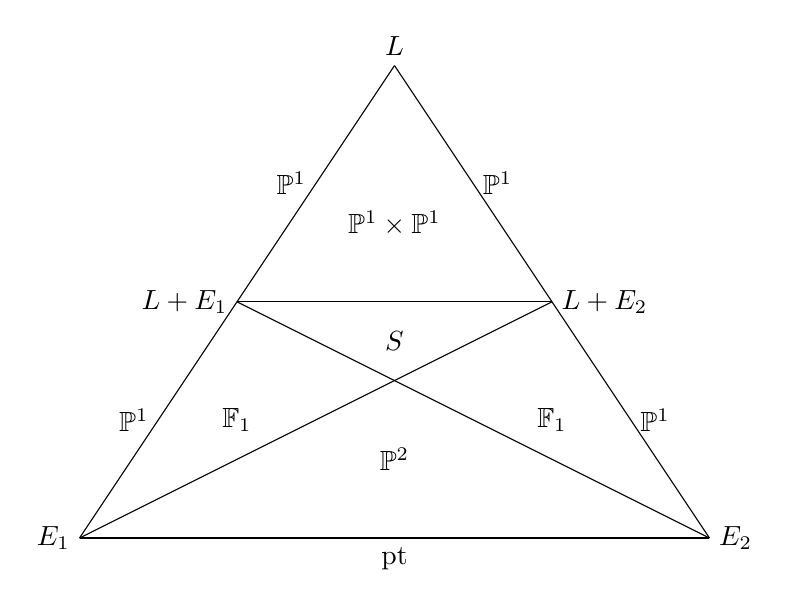
\begin{tikzpicture}
	\draw (-4,0)node[left]{$ E_1 $}--(0,0)node[below]{pt}--(4,0)node[right]{$ E_2 $};
	\draw(-4,0)--(-3,1.5)node[left]{$ \mathbb{P}^1 $}--(-2,3)node[left]{$ L+E_1 $}--(-1,4.5)node[left]{$ \mathbb{P}^1 $}--(0,6)node[above]{$ L $};
	\draw(4,0)--(3,1.5)node[right]{$ \mathbb{P}^1 $}--(2,3)node[right]{$ L+E_2 $}--(1,4.5)node[right]{$ \mathbb{P}^1 $}--(0,6);
	\draw (-2,3)--(4,0);
	\draw (2,3)--(-4,0);
	\draw (-2,3)--(2,3);
	\draw (0,2.5)node{$ S $};
	\draw (2,1.5)node{$ \mathbb{F}_1 $};
	\draw (-2,1.5)node{$ \mathbb{F}_1 $};
	\draw (0,4)node{$ \mathbb{P}^1\times \mathbb{P}^1 $};
	\draw (0,1)node{$ \mathbb{P}^2 $};
\end{tikzpicture}

\subsection{Find the path}
\begin{lem}
	Let $ \phi:X\to S $ and $ \psi :Y\to T  $ be two MMP related MFS corresponding to two klt projective varieies $ (X,B_X) $ and $ (Y,B_Y) $. Then we may find a smooth projective variety $ W $, two biratinal contractions $ f:W\dashrightarrow X $ and $ g:W\dashrightarrow Y $, a klt pair $ (Z,B_Z) $, an ample $ \mathbb{Q} $-divisor $ A $ on $ X $ and a two dimensional rational affine subspace $ V $ of $ \mathrm{WDiv}_\mathbb{R}(W) $ such that 
	\begin{enumerate}[1)]
		\item If $ D\in \mathcal{L}_A(V) $ then $ D-B_Z $ is ample;
		\item $ \mathcal{A}_{A,\phi\circ f} $ and $ \mathcal{A}_{A,\psi\circ g} $ are not contained in the boundary of $ \mathcal{L}_A(V) $;
		\item $ V $ satisfy \ref{finite ample models};
		\item $ \mathcal{C}_{A,f} $ and $ \mathcal{C}_{A,g} $ are two dimensional;
		\item $ \mathcal{C}_{A,\phi\circ f} $ and $ \mathcal{C}_{A,\psi\circ g} $ are one dimensional.
	\end{enumerate}
\end{lem}

By the lemma we have a 'map', and hence we can find a path:

\begin{proof}[Proof of the main theorem]
	Pick $ D_0\in \mathcal{A}_{A,\phi\circ f} $  and $ D_1\in \mathcal{C}_{A,g} $ belonging to the interior of $ \mathcal{L}_A(V) $. As $ V $ is two dimensional, removing $ D_0 $ and $ D_1 $ divides the boundary of $ \mathcal{E}_A(V) $ into two parts. The part which consists entirely of divisors which are not big is contained in the interior of $ \mathcal{L}_A(V) $. Consider tracing this boundary from $ D_0 $ to $ D_1 $. Then there are finitely many $ 2\leqslant i\leqslant N $ points $ D_i $ which are contained in more than two polytopes $ \mathcal{C}_{A,f_i}(V) $. Each point $ D_i $ gives a link.
\end{proof}


\end{document}
